%-------------------------
%big-picture
%(c) H.Buchmann FHNW 2008
%$Id$
%export TEXINPUTS=${HOME}/fhnw/edu/:${HOME}/fhnw/edu/tinL/config/latex:${HOME}/fhnw/edu/config//:
%-------------------------
\documentclass{beamer}
\usepackage{latex/beamer}
%---------------------
%local defines
%(c) H.Buchmann FHNW 2009
%$Id$
%---------------------
\newcommand{\target} {\beaglebone\xspace}
\newcommand{\targetS}{{\bf BBG}\xspace}
\newcommand{\host}   {{\em Host}\xspace}
\newcommand{\targetroot} {{\bf target-root}\xspace}
\newcommand{\kernel} {{\bf kernel}\xspace}
\renewcommand{\c}{{\bf C}\xspace}
\newcommand{\cpp}{{\bf C++}\xspace}
\newcommand{\posix}{{\bf POSIX}\xspace}

\input{/home/buchmann/latex/dirtree/dirtree.tex}

\title{Partitionen}
\begin{document}

\newcommand{\distro}{sd-2016-09-28.img.gz}

\frame{\titlepage}

\begin{frame}{Ziele}{alles ist ein File: {\em stream of bits}}
 \begin{itemize}
  \item Tr�ger von Filesystemen
  \item Aufbau
  \begin{itemize}
   \item MBR: Master Boot Record
  \end{itemize}
  \item Herstellung
 \end{itemize}
 \remark{Alles ist ein File  {\em stream of bits}}
\end{frame}

\begin{frame}{Partitionen Termiologie \linux}{Tr�ger von Filesystemen}
 \begin{itemize}
  \item Festplatte \cod{ls /dev/sd*}
  \begin{itemize}
   \item \cod{/dev/sd{\em X}}, \cod{{\em X}=a,b,c ...}
   \item Partitionen 
   \begin{itemize}
     \item \cod{/dev/sd{\em X}{\em N}} \cod{{\em N}=1,2,3 ...} 
   \end{itemize} 
  \end{itemize}
  \item SD-Karten \cod{ls /dev/mmcblk*}
  \begin{itemize}
   \item \cod{/dev/mmcblk{\em N}} \cod{{\em N}=0,1,2 ...}
   \item Partitionen
   \begin{itemize}
     \item \cod{/dev/mmcblk{\em N}p{\em N}} \cod{{\em N}=0,1,2 ...} 
   \end{itemize} 
   
  \end{itemize}
 \end{itemize}
\end{frame} 

\section{Massenspeicher}
\begin{frame}{Massenspeicher}{non volatile}
 \begin{block}{Arten}
  \begin{itemize}
   \item mechanische Festplatten
   \item SSD Karten
   \item SD-Karten
   \item Flash
   \item ...
  \end{itemize}
 \end{block}
 \begin{block}{Typisch}
  \begin{itemize}
   \item Zugriff relativ langsam
   \item Blockorientiert 
   \begin{itemize}
    \item Mehrere Bits/Bytespro Zugriff
   \end{itemize}
  \end{itemize}
 \end{block}
\end{frame}

\begin{frame}[fragile]{Massenspeicher}{Blocks/Sektoren}
\begin{lstlisting}
 typedef unsigned char Sector[512]; 
 Sector MassStorage[N];
\end{lstlisting}
\remark{Ein langer Array von Sektoren}
\begin{center}
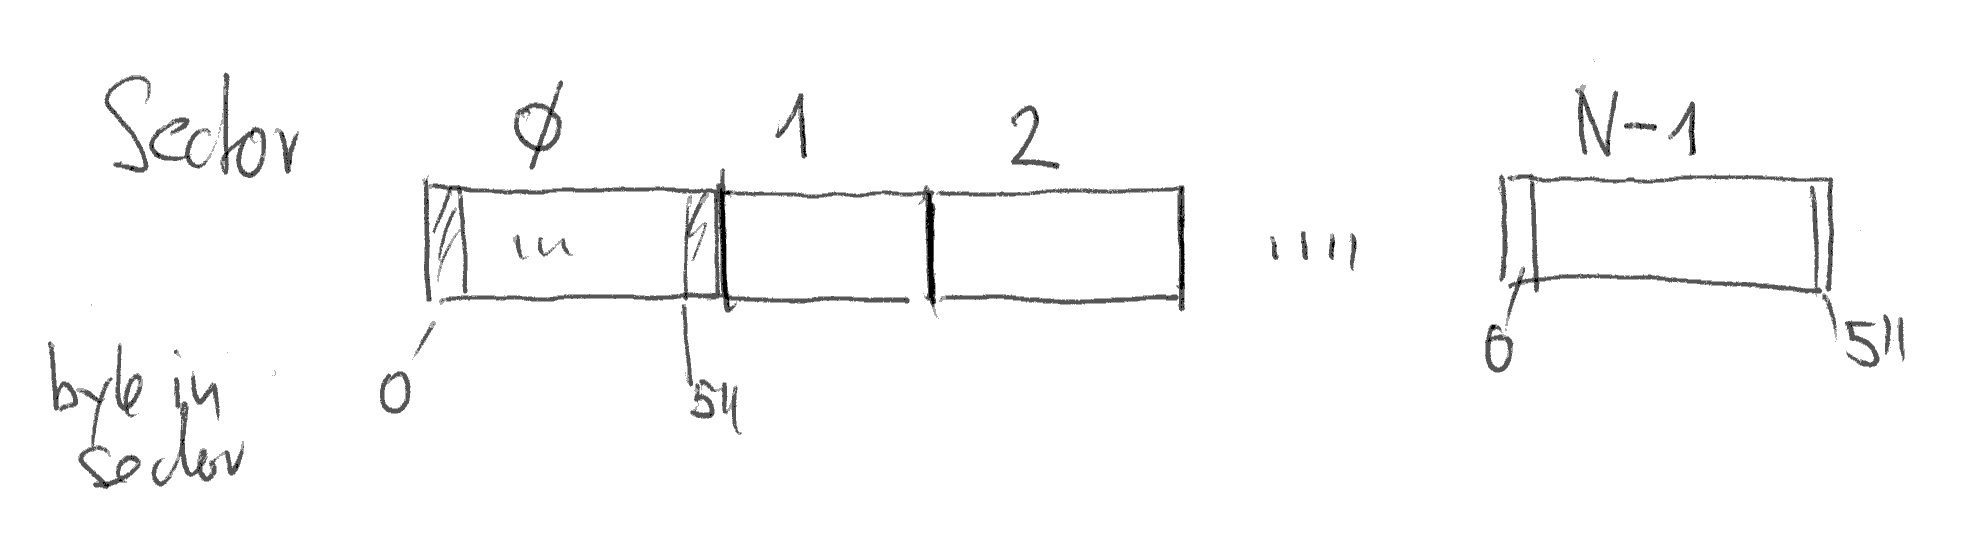
\includegraphics[width=0.875\textwidth]{array-of-sector.jpg}
\end{center}
\end{frame}

\begin{frame}[fragile]{Der Befehl \cod{dd}}{Vorsicht}
\begin{lstlisting}[language=bash]
dd if=/dev/mmcblk0 count=1|hexdump -C        
  # first sector to stdout
dd if=/dev/mmcblk0 skip=1 count=1|hexdump -C 
  # second sector to stdout
dd if=/dev/mmcblk0 of=mbr.bin count=1        
  # copy sector to mbr.bin
\end{lstlisting}
\end{frame}

\section{MBR}
\begin{frame}[fragile]{MBR: Master Boot Record}{Verzeichnis der Partionen}
\begin{lstlisting}[language=bash]
dd if=/dev/mmcblk0 count=1|hexdump -C
\end{lstlisting}
{\scriptsize
\begin{verbatim}
00000000  00 00 00 00 00 00 00 00  00 00 00 00 00 00 00 00  |................|
*
000001b0  00 00 00 00 00 00 00 00  ba 23 8e d6 00 00 00 00  |.........#......|
000001c0  01 20 0b 03 10 1f 00 08  00 00 00 00 04 00 00 00  |. ..............|
000001d0  01 20 83 03 50 df 00 08  04 00 00 70 71 00 00 00  |. ..P......pq...|
000001e0  00 00 00 00 00 00 00 00  00 00 00 00 00 00 00 00  |................|
000001f0  00 00 00 00 00 00 00 00  00 00 00 00 00 00 55 aa  |..............U.|
00000200
\end{verbatim}
}

{\scriptsize\url{technet.microsoft.com/en-us/library/cc976786.aspx}}

\end{frame}

\section{Distribution}
\begin{frame}[fragile]{Alles ist ein File}{und umgekehrt}
\begin{itemize}
 \item Der File \cod{\distro}
 ist das Bild einer ganzen SD-Karte
 \item Mache SD-Karte
 \begin{itemize}
  \item Kopiere {\tiny\url{sourceforge.net/projects/fhnw-tinl/files/{\distro}/download}} 
  \item entzippe
  \item kopiere
  \begin{lstlisting}
dd if=distro.img of=/dev/sd-card
  \end{lstlisting}
  \cod{sd-card} typ \cod{mmcblk\em{N}} $N=0|1 ..$
 \end{itemize}
 \remark{Alles mit {\em pipes}}
 
\end{itemize}

\end{frame}
\end{document}

